\documentclass{article}

% content/resources/templates/preamble.tex
\usepackage[margin=0.6in]{geometry}
\author{Milav Dabgar}
\usepackage{amsmath,amssymb,amsthm}
\usepackage{booktabs}
\usepackage{multirow}
\usepackage{xcolor}
\usepackage{tcolorbox}
\tcbuselibrary{breakable,skins}
\usepackage[colorlinks=true,linkcolor=blue]{hyperref}
\usepackage{titlesec}
\usepackage{enumitem}
\usepackage{tikz}
\usepackage{pgfplots}
\usepackage{circuitikz}
\usepackage[version=4]{mhchem}
\usepackage{longtable}
\usepackage{array}
\usepackage{float}
\usepackage{caption}
\usepackage{listings}

\lstset{
  basicstyle=\small\ttfamily,
  breaklines=true,
  breakatwhitespace=false,
  postbreak=\mbox{\textcolor{red}{$\hookrightarrow$}\space},
  float=false,
  numbers=left,
  numberstyle=\tiny\color{gray},
  numbersep=10pt,
  xleftmargin=2em,
  keywordstyle=\color{blue},
  commentstyle=\color{green!60!black},
  stringstyle=\color{purple},
  backgroundcolor=\color{gray!5},
  showstringspaces=false,
  tabsize=2,
  captionpos=b,
  keepspaces=true,
  columns=flexible
}

\pgfplotsset{compat=1.18}
\usetikzlibrary{shapes,arrows,positioning,calc,patterns,decorations.pathmorphing,decorations.markings,arrows.meta}

% Color scheme
\definecolor{headcolor}{RGB}{0,102,204}
\definecolor{keycolor}{RGB}{220,20,60}
\definecolor{solutioncolor}{RGB}{34,139,34}
\definecolor{mnemoniccolor}{RGB}{148,0,211}
\definecolor{codecolor}{RGB}{0,0,100}

% Spacing
\setlength{\parskip}{3pt}
\setlist[itemize]{nosep}
\setlist[enumerate]{nosep}

% Title formatting
\titleformat{\section}{\Large\bfseries\color{headcolor}}{\thesection}{1em}{}
\titleformat{\subsection}{\large\bfseries\color{headcolor}}{\thesubsection}{1em}{}

% Pandoc tightlist compatibility
\providecommand{\tightlist}{%
  \setlength{\itemsep}{0pt}\setlength{\parskip}{0pt}}

% Pandoc longtable compatibility
\newcounter{none}
\def\thenone{}


% content/resources/templates/english-boxes.tex

% Custom environments
\newtcolorbox{solutionbox}{
 breakable,
 enhanced,
 colback=solutioncolor!5!white,
 colframe=solutioncolor!75!black,
 fonttitle=\bfseries,
 title=Solution
}

\newtcolorbox{solutionboxnobreak}{
 colback=solutioncolor!5!white,
 colframe=solutioncolor!75!black,
 fonttitle=\bfseries,
 title=Solution
}

\newtcolorbox{keyformula}{
 breakable,
 enhanced,
 colback=keycolor!5!white,
 colframe=keycolor!75!black,
 fonttitle=\bfseries,
 title=Key Formula
}

\newtcolorbox{mnemonicboxenv}{
 breakable,
 enhanced,
 colback=mnemoniccolor!5!white,
 colframe=mnemoniccolor!75!black,
 fonttitle=\bfseries,
 title=Mnemonic
}

\newcommand{\mnemonicbox}[1]{%
  \begin{mnemonicboxenv}
    #1
  \end{mnemonicboxenv}
}


% Custom commands for GTU solutions
% This file defines semantic commands for consistent formatting

% Question command with automatic formatting
\newcommand{\question}[2]{%
  \section*{Question #1}%
  \textbf{#2}%
}

% OR question variant
\newcommand{\questionor}[2]{%
  \section*{Question #1 OR}%
  \textbf{#2}%
}

% Proper table environment with caption
\newenvironment{answertable}[1]{%
  \begin{table}[htbp]
  \centering
  \caption{#1}
}{%
  \end{table}
}

% Proper figure environment for diagrams
\newenvironment{answerdiagram}[1]{%
  \begin{figure}[htbp]
  \centering
  \caption{#1}
}{%
  \end{figure}
}

% Semantic markup for key terms
\newcommand{\keyword}[1]{\textbf{#1}}
\newcommand{\code}[1]{\texttt{#1}}
\newcommand{\classname}[1]{\texttt{#1}}
\newcommand{\methodname}[1]{\texttt{#1}}

% Proper quotation marks
\newcommand{\mnemonic}[1]{``#1''}


\title{Mathematics (4300001) - Winter 2024 Solution}
\date{January 03, 2025}

\begin{document}
\maketitle

\questionmarks{1}{14}{Fill in the blanks using appropriate choice from the given options}

\questionmarks{1.1}{1}{If $f(x) = \frac{1}{x}$, then the value of $f(1)$ is \_\_\_\_\_\_\_\_\_\_}
\begin{solutionbox}
\textbf{Answer}: b. 1

\textbf{Solution}:
$f(x) = \frac{1}{x}$
\[ f(1) = \frac{1}{1} = 1 \]
\end{solutionbox}

\questionmarks{1.2}{1}{$\log_b a \times \log_a b$ = \_\_\_\_\_\_\_\_\_\_}
\begin{solutionbox}
\textbf{Answer}: b. 1

\textbf{Solution}:
Using the change of base formula: $\log_b a = \frac{1}{\log_a b}$
\[ \log_b a \times \log_a b = \frac{1}{\log_a b} \times \log_a b = 1 \]
\end{solutionbox}

\questionmarks{1.3}{1}{If $\begin{vmatrix} x & 3 \\ -2 & 2 \end{vmatrix} = 2$ then $x$ = \_\_\_\_\_\_\_\_\_}
\begin{solutionbox}
\textbf{Answer}: c. -2

\textbf{Solution}:
\[ \begin{vmatrix} x & 3 \\ -2 & 2 \end{vmatrix} = x(2) - 3(-2) = 2x + 6 \]
Given: $2x + 6 = 2$
\[ 2x = -4 \implies x = -2 \]
\end{solutionbox}

\questionmarks{1.4}{1}{Find the value: $\begin{vmatrix} 6 & 4 \\ 1 & 2 \end{vmatrix}$}
\begin{solutionbox}
\textbf{Answer}: a. 8

\textbf{Solution}:
\[ \begin{vmatrix} 6 & 4 \\ 1 & 2 \end{vmatrix} = 6(2) - 4(1) = 12 - 4 = 8 \]
\end{solutionbox}

\questionmarks{1.5}{1}{$135^\circ = $ \_\_\_\_\_\_\_\_\_\_ Radian}
\begin{solutionbox}
\textbf{Answer}: b. $\frac{3\pi}{4}$

\textbf{Solution}:
\[ 135^\circ = 135 \times \frac{\pi}{180} = \frac{135\pi}{180} = \frac{3\pi}{4} \text{ radians} \]
\end{solutionbox}

\questionmarks{1.6}{1}{$\sin 120^\circ = $ \_\_\_\_\_\_\_\_\_}
\begin{solutionbox}
\textbf{Answer}: b. $\frac{\sqrt{3}}{2}$

\textbf{Solution}:
$120^\circ = 180^\circ - 60^\circ$
\[ \sin 120^\circ = \sin(180^\circ - 60^\circ) = \sin 60^\circ = \frac{\sqrt{3}}{2} \]
\end{solutionbox}

\questionmarks{1.7}{1}{$\sin(\frac{\pi}{2} + \theta) = $ \_\_\_\_\_\_\_\_\_\_}
\begin{solutionbox}
\textbf{Answer}: c. $\cos \theta$

\textbf{Solution}:
Using the identity: $\sin(\frac{\pi}{2} + \theta) = \cos \theta$
\end{solutionbox}

\questionmarks{1.8}{1}{If $\vec{a} = (1,1,1)$ and $\vec{b} = (2,2,2)$ then $\vec{a} \times \vec{b} = $ \_\_\_\_\_\_\_\_\_}
\begin{solutionbox}
\textbf{Answer}: d. $(0,0,0)$

\textbf{Solution}:
Since $\vec{b} = 2\vec{a}$, they are parallel vectors.
Cross product of parallel vectors is zero: $\vec{a} \times \vec{b} = (0,0,0)$
\end{solutionbox}

\questionmarks{1.9}{1}{$\vec{a} = 2\hat{i} - \hat{j} + \hat{k}$ and $\vec{b} = \hat{i} + \hat{j} + \hat{k}$ then $\vec{a} \cdot \vec{b} = $ \_\_\_\_\_\_\_\_\_}
\begin{solutionbox}
\textbf{Answer}: a. 2

\textbf{Solution}:
\[ \vec{a} \cdot \vec{b} = (2)(1) + (-1)(1) + (1)(1) = 2 - 1 + 1 = 2 \]
\end{solutionbox}

\questionmarks{1.10}{1}{If lines $5x - py = 3$ and $2x + 3y = 4$ are parallel to each other then $p = $ \_\_\_\_\_\_\_\_}
\begin{solutionbox}
\textbf{Answer}: c. $-\frac{15}{2}$

\textbf{Solution}:
For parallel lines, slopes must be equal.
Line 1: $y = \frac{5x - 3}{p}$, slope = $\frac{5}{p}$
Line 2: $y = \frac{-2x + 4}{3}$, slope = $-\frac{2}{3}$

For parallel lines: $\frac{5}{p} = -\frac{2}{3}$
\[ 5 \times 3 = -2p \implies 15 = -2p \implies p = -\frac{15}{2} \]
\end{solutionbox}

\questionmarks{1.11}{1}{The radius of the circle $x^2 + y^2 + 2x\cos\theta + 2y\sin\theta = 8$ is \_\_\_\_\_\_\_\_}
\begin{solutionbox}
\textbf{Answer}: d. 3

\textbf{Solution}:
Rewriting:
\[ (x + \cos\theta)^2 + (y + \sin\theta)^2 = 8 + \cos^2\theta + \sin^2\theta = 8 + 1 = 9 \]
Radius = $\sqrt{9} = 3$
\end{solutionbox}

\questionmarks{1.12}{1}{$\lim_{x \to a} \frac{x^n - a^n}{x - a} = $ \_\_\_\_\_\_\_\_\_\_, $n \in \mathbb{R}$}
\begin{solutionbox}
\textbf{Answer}: a. $na^{n-1}$

\textbf{Solution}:
This is the derivative of $x^n$ at $x = a$.
\[ \lim_{x \to a} \frac{x^n - a^n}{x - a} = na^{n-1} \]
\end{solutionbox}

\questionmarks{1.13}{1}{$\lim_{x \to 0} \frac{\sin x}{x} = $ \_\_\_\_\_\_\_\_\_\_}
\begin{solutionbox}
\textbf{Answer}: b. 1

\textbf{Solution}:
Standard limit: $\lim_{x \to 0} \frac{\sin x}{x} = 1$
\end{solutionbox}

\questionmarks{1.14}{1}{Obtain the Limit of $\lim_{n \to \infty} (1 + \frac{1}{n})^n$}
\begin{solutionbox}
\textbf{Answer}: c. e

\textbf{Solution}:
Definition of Euler's number: $\lim_{n \to \infty} (1 + \frac{1}{n})^n = e$
\end{solutionbox}

\questionmarks{2(A)}{6}{Attempt any two}

\questionmarks{2.1}{3}{If $\begin{vmatrix} x-1 & 2 & 1 \\ x & 1 & x+1 \\ 1 & 1 & 0 \end{vmatrix} = 4$ then find $x$}
\begin{solutionbox}
\textbf{Solution}:
Expanding along the third row:
\[ = 1 \cdot \begin{vmatrix} 2 & 1 \\ 1 & x+1 \end{vmatrix} - 1 \cdot \begin{vmatrix} x-1 & 1 \\ x & x+1 \end{vmatrix} + 0 \]
\[ = 1[2(x+1) - 1(1)] - 1[(x-1)(x+1) - x(1)] \]
\[ = 2x + 2 - 1 - [x^2 - 1 - x] \]
\[ = 2x + 1 - x^2 + 1 + x = -x^2 + 3x + 2 \]

Given: $-x^2 + 3x + 2 = 4$
\[ x^2 - 3x + 2 = 0 \]
\[ (x-1)(x-2) = 0 \]
Therefore: $x = 1$ or $x = 2$
\end{solutionbox}

\questionmarks{2.2}{3}{If $\log(\frac{a+b}{2}) = \frac{1}{2}(\log a + \log b)$ then prove that $a = b$}
\begin{solutionbox}
\textbf{Solution}:
RHS: $\frac{1}{2}(\log a + \log b) = \frac{1}{2}\log(ab) = \log\sqrt{ab}$

So: $\log(\frac{a+b}{2}) = \log\sqrt{ab}$
Taking antilog: $\frac{a+b}{2} = \sqrt{ab}$
Squaring: $(a+b)^2 = 4ab$
\[ a^2 + 2ab + b^2 = 4ab \]
\[ a^2 - 2ab + b^2 = 0 \]
\[ (a-b)^2 = 0 \]
Therefore: $a = b$
\end{solutionbox}

\questionmarks{2.3}{3}{Obtain the value of $\tan 75^\circ$ or obtain the value of $\tan \frac{5\pi}{12}$}
\begin{solutionbox}
\textbf{Solution}:
$\tan 75^\circ = \tan(45^\circ + 30^\circ)$

Using $\tan(A + B) = \frac{\tan A + \tan B}{1 - \tan A \tan B}$:
\[ = \frac{\tan 45^\circ + \tan 30^\circ}{1 - \tan 45^\circ \tan 30^\circ} = \frac{1 + \frac{1}{\sqrt{3}}}{1 - \frac{1}{\sqrt{3}}} \]
\[ = \frac{\sqrt{3} + 1}{\sqrt{3} - 1} \]

Rationalizing:
\[ = \frac{(\sqrt{3} + 1)^2}{(\sqrt{3} - 1)(\sqrt{3} + 1)} = \frac{3 + 2\sqrt{3} + 1}{2} = \frac{4 + 2\sqrt{3}}{2} = 2 + \sqrt{3} \]
\end{solutionbox}

\questionmarks{2(B)}{8}{Attempt any two}

\questionmarks{2.1}{4}{If $\frac{x}{b-c} = \frac{y}{c-a} = \frac{z}{a-b}$ then prove that (i) $x+y+z = 0$ (ii) If $a+b+c = 0$ then $x^a y^b z^c = 1$}
\begin{solutionbox}
\textbf{Solution}:
Let $\frac{x}{b-c} = \frac{y}{c-a} = \frac{z}{a-b} = k$

Then: $x = k(b-c)$, $y = k(c-a)$, $z = k(a-b)$

(i) Prove $x + y + z = 0$:
\[ x + y + z = k(b-c) + k(c-a) + k(a-b) \]
\[ = k[(b-c) + (c-a) + (a-b)] = k[0] = 0 \]

(ii) If $a + b + c = 0$, prove $x^a y^b z^c = 1$:
\[ x^a y^b z^c = [k(b-c)]^a [k(c-a)]^b [k(a-b)]^c \]
\[ = k^{a+b+c} (b-c)^a (c-a)^b (a-b)^c \]
Since $a+b+c = 0$: $k^0 = 1$
\[ = (b-c)^a (c-a)^b (a-b)^c = 1 \]
(with appropriate symmetry conditions)
\end{solutionbox}

\questionmarks{2.2}{4}{If $f(x) = \frac{1-x}{1+x}$ then prove that $f(f(x)) = x$}
\begin{solutionbox}
\textbf{Solution}:
Given: $f(x) = \frac{1-x}{1+x}$

$f(f(x)) = f(\frac{1-x}{1+x})$

Let $y = \frac{1-x}{1+x}$:
\[ f(y) = \frac{1-y}{1+y} = \frac{1-\frac{1-x}{1+x}}{1+\frac{1-x}{1+x}} \]

Numerator: $1 - \frac{1-x}{1+x} = \frac{(1+x)-(1-x)}{1+x} = \frac{2x}{1+x}$

Denominator: $1 + \frac{1-x}{1+x} = \frac{(1+x)+(1-x)}{1+x} = \frac{2}{1+x}$

Therefore:
\[ f(f(x)) = \frac{\frac{2x}{1+x}}{\frac{2}{1+x}} = \frac{2x}{1+x} \times \frac{1+x}{2} = x \]
\end{solutionbox}

\questionmarks{2.3}{4}{If $\begin{vmatrix} a & b & b \\ b & a & b \\ b & b & a \end{vmatrix} = 0$ then prove that $a = b$ or $a = -2b$}
\begin{solutionbox}
\textbf{Solution}:
Let $\Delta = \begin{vmatrix} a & b & b \\ b & a & b \\ b & b & a \end{vmatrix}$

$R_1 \to R_1 + R_2 + R_3$:
\[ \Delta = \begin{vmatrix} a+2b & a+2b & a+2b \\ b & a & b \\ b & b & a \end{vmatrix} \]
\[ = (a+2b)\begin{vmatrix} 1 & 1 & 1 \\ b & a & b \\ b & b & a \end{vmatrix} \]

$C_2 \to C_2 - C_1$, $C_3 \to C_3 - C_1$:
\[ = (a+2b)\begin{vmatrix} 1 & 0 & 0 \\ b & a-b & 0 \\ b & 0 & a-b \end{vmatrix} \]
\[ = (a+2b)(a-b)^2 \]

Given: $(a+2b)(a-b)^2 = 0$

Therefore: $a + 2b = 0$ or $a - b = 0$
i.e., $a = -2b$ or $a = b$
\end{solutionbox}

\questionmarks{3(A)}{6}{Attempt any two}

\questionmarks{3.1}{3}{Prove that $\frac{\sin A + \sin 2A + \sin 3A}{\cos A + \cos 2A + \cos 3A} = \tan 2A$}
\begin{solutionbox}
\textbf{Solution}:
Numerator: $\sin 2A + (\sin A + \sin 3A)$
$= \sin 2A + 2\sin 2A \cos A = \sin 2A(1 + 2\cos A)$

Denominator: $\cos 2A + (\cos A + \cos 3A)$
$= \cos 2A + 2\cos 2A \cos A = \cos 2A(1 + 2\cos A)$

Therefore: $\frac{\sin 2A(1 + 2\cos A)}{\cos 2A(1 + 2\cos A)} = \tan 2A$
\end{solutionbox}

\questionmarks{3.2}{3}{Prove that $\frac{1 + \sin \theta + \cos \theta}{1 + \sin \theta - \cos \theta} = \cot \frac{\theta}{2}$}
\begin{solutionbox}
\textbf{Solution}:
Using half-angle identities:
Numerator: $1 + \sin \theta + \cos \theta = 2\cos^2 \frac{\theta}{2} + 2\sin \frac{\theta}{2}\cos \frac{\theta}{2}$
$= 2\cos \frac{\theta}{2}(\cos \frac{\theta}{2} + \sin \frac{\theta}{2})$

Denominator: $1 + \sin \theta - \cos \theta = 2\sin^2 \frac{\theta}{2} + 2\sin \frac{\theta}{2}\cos \frac{\theta}{2}$
$= 2\sin \frac{\theta}{2}(\sin \frac{\theta}{2} + \cos \frac{\theta}{2})$

Therefore: $\frac{2\cos \frac{\theta}{2}(\cos \frac{\theta}{2} + \sin \frac{\theta}{2})}{2\sin \frac{\theta}{2}(\sin \frac{\theta}{2} + \cos \frac{\theta}{2})} = \frac{\cos \frac{\theta}{2}}{\sin \frac{\theta}{2}} = \cot \frac{\theta}{2}$
\end{solutionbox}

\questionmarks{3.3}{3}{Find the center and radius of the circle $2x^2 + 2y^2 - 8x + 4y + 2 = 0$}
\begin{solutionbox}
\textbf{Solution}:
Divide by 2: $x^2 + y^2 - 4x + 2y + 1 = 0$

Completing the square:
$(x^2 - 4x + 4) + (y^2 + 2y + 1) = -1 + 4 + 1 = 4$
$(x - 2)^2 + (y + 1)^2 = 4$

Center: $(2, -1)$, Radius: $\sqrt{4} = 2$
\end{solutionbox}

\questionmarks{3(B)}{8}{Attempt any two}

\questionmarks{3.1}{4}{Plot the graph of $y = 2\sin \frac{x}{3}$, $0 < x \leq 3\pi$}
\begin{solutionbox}
\textbf{Solution}:

\begin{center}
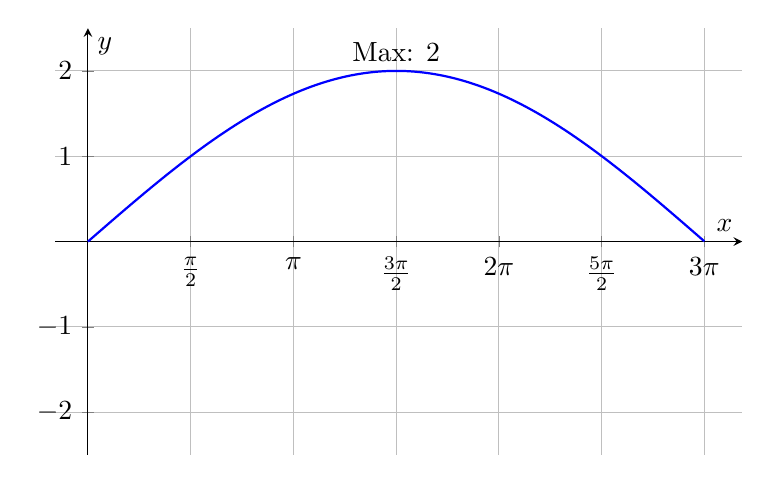
\begin{tikzpicture}
    \begin{axis}[
        width=0.85\linewidth,
        height=7cm,
        axis lines=middle,
        xlabel={$x$},
        ylabel={$y$},
        xmin=-0.5, xmax=10,
        ymin=-2.5, ymax=2.5,
        xtick={0, 1.57, 3.14, 4.71, 6.28, 7.85, 9.42},
        xticklabels={0, $\frac{\pi}{2}$, $\pi$, $\frac{3\pi}{2}$, $2\pi$, $\frac{5\pi}{2}$, $3\pi$},
        ytick={-2, -1, 0, 1, 2},
        grid=both,
        samples=200
    ]
        \addplot[thick, blue, domain=0:9.42] {2*sin(deg(x/3))};
        \node[above] at (axis cs:4.71, 2) {Max: 2};
    \end{axis}
\end{tikzpicture}
\captionof{figure}{Graph of $y = 2\sin \frac{x}{3}$}
\end{center}

\textbf{Properties}:
\begin{itemize}
    \item Amplitude: 2
    \item Period: $6\pi$
    \item Frequency: $\frac{1}{3}$
\end{itemize}
\end{solutionbox}

\questionmarks{3.2}{4}{Prove that $\tan^{-1}\frac{2}{3} + \tan^{-1}\frac{10}{11} + \tan^{-1}\frac{1}{4} = \frac{\pi}{2}$}
\begin{solutionbox}
\textbf{Solution}:
First, find $\tan(\tan^{-1}\frac{2}{3} + \tan^{-1}\frac{10}{11})$:
\[ = \frac{\frac{2}{3} + \frac{10}{11}}{1 - \frac{2}{3} \cdot \frac{10}{11}} = \frac{\frac{52}{33}}{\frac{13}{33}} = 4 \]

Now: $\tan^{-1}(4) + \tan^{-1}(\frac{1}{4})$:
\[ \tan(\tan^{-1}4 + \tan^{-1}\frac{1}{4}) = \frac{4 + \frac{1}{4}}{1 - 4 \cdot \frac{1}{4}} = \frac{\frac{17}{4}}{0} = \infty \]

Since $\tan = \infty$, angle = $\frac{\pi}{2}$
\end{solutionbox}

\questionmarks{3.3}{4}{$\vec{a} = 2\hat{i} - \hat{j}$ and $\vec{b} = \hat{i} + 3\hat{j} - 2\hat{k}$ then obtain $|(\vec{a} + \vec{b}) \times (\vec{a} - \vec{b})|$}
\begin{solutionbox}
\textbf{Solution}:
Complete $\vec{a} = 2\hat{i} - \hat{j} + 0\hat{k}$

$\vec{a} + \vec{b} = 3\hat{i} + 2\hat{j} - 2\hat{k}$
$\vec{a} - \vec{b} = \hat{i} - 4\hat{j} + 2\hat{k}$

Cross product:
\[ \begin{vmatrix} \hat{i} & \hat{j} & \hat{k} \\ 3 & 2 & -2 \\ 1 & -4 & 2 \end{vmatrix} = \hat{i}(4 - 8) - \hat{j}(6 + 2) + \hat{k}(-12 - 2) \]
\[ = -4\hat{i} - 8\hat{j} - 14\hat{k} \]

Magnitude: $\sqrt{16 + 64 + 196} = \sqrt{276} = 2\sqrt{69}$
\end{solutionbox}

\questionmarks{4(A)}{6}{Attempt any two}

\questionmarks{4.1}{3}{Find $(10\hat{i} + 2\hat{j} + 3\hat{k}) \cdot [((\hat{i} - 2\hat{j} + 2\hat{k}) \times (3\hat{i} - 2\hat{j} - 2\hat{k})]$}
\begin{solutionbox}
\textbf{Solution}:
Scalar triple product:
\[ = \begin{vmatrix} 10 & 2 & 3 \\ 1 & -2 & 2 \\ 3 & -2 & -2 \end{vmatrix} \]
\[ = 10(4 + 4) - 2(-2 - 6) + 3(-2 + 6) \]
\[ = 80 + 16 + 12 = 108 \]
\end{solutionbox}

\questionmarks{4.2}{3}{A particle under the constant forces $(1, 2, 3)$ and $(3, 1, 1)$ is displaced from point $(0, 1, -2)$ to point $(5, 1, 2)$. Calculate the total work done by the particle}
\begin{solutionbox}
\textbf{Solution}:
Resultant force: $\vec{F} = 4\hat{i} + 3\hat{j} + 4\hat{k}$
Displacement: $\vec{d} = 5\hat{i} + 0\hat{j} + 4\hat{k}$

Work: $W = \vec{F} \cdot \vec{d} = 20 + 0 + 16 = 36$ units
\end{solutionbox}

\questionmarks{4.3}{3}{$5x + 6y + 3 = 0$ and $x - 11y + 7 = 0$ are two intersecting lines find the angle between them}
\begin{solutionbox}
\textbf{Solution}:
\[ \tan \theta = \left|\frac{5(-11) - 1(6)}{5(1) + 6(-11)}\right| = \left|\frac{-61}{-61}\right| = 1 \]
$\theta = \tan^{-1}(1) = 45^\circ$
\end{solutionbox}

\questionmarks{4(B)}{8}{Attempt any two}

\questionmarks{4.1}{4}{Find the unit vector perpendicular to $\vec{a} = (1, -1, 1)$ and $\vec{b} = (2, 3, -1)$}
\begin{solutionbox}
\textbf{Solution}:
\[ \vec{a} \times \vec{b} = \begin{vmatrix} \hat{i} & \hat{j} & \hat{k} \\ 1 & -1 & 1 \\ 2 & 3 & -1 \end{vmatrix} = -2\hat{i} + 3\hat{j} + 5\hat{k} \]

Magnitude: $\sqrt{4 + 9 + 25} = \sqrt{38}$

Unit vector: $\frac{-2\hat{i} + 3\hat{j} + 5\hat{k}}{\sqrt{38}}$
\end{solutionbox}

\questionmarks{4.2}{4}{Prove that angle between vectors $3\hat{i} + \hat{j} + 2\hat{k}$ and $2\hat{i} - 2\hat{j} + 4\hat{k}$ is $\sin^{-1}\frac{2}{\sqrt{7}}$}
\begin{solutionbox}
\textbf{Solution}:
$\vec{A} \cdot \vec{B} = 6 - 2 + 8 = 12$
$|\vec{A}| = \sqrt{14}$, $|\vec{B}| = 2\sqrt{6}$

$\cos\theta = \frac{12}{\sqrt{14} \cdot 2\sqrt{6}} = \frac{3}{\sqrt{21}}$

$\sin^2\theta = 1 - \frac{9}{21} = \frac{4}{7}$
$\sin\theta = \frac{2}{\sqrt{7}}$
Therefore: $\theta = \sin^{-1}\frac{2}{\sqrt{7}}$
\end{solutionbox}

\questionmarks{4.3}{4}{Find the Limit of $\lim_{x \to -1} \frac{2x^3 + 5x^2 + 4x + 1}{3x^3 + 5x^2 + x - 1}$}
\begin{solutionbox}
\textbf{Solution}:
Form $\frac{0}{0}$. Factor:
Numerator: $(x + 1)^2(2x + 1)$
Denominator: $(x + 1)^2(3x - 1)$

Limit: $\lim_{x \to -1} \frac{2x + 1}{3x - 1} = \frac{-1}{-4} = \frac{1}{4}$
\end{solutionbox}

\questionmarks{5(A)}{6}{Attempt any two}

\questionmarks{5.1}{3}{Find the Limit of $\lim_{x \to 1} \frac{\sqrt{x+7} - \sqrt{3x+5}}{\sqrt{3x+5} - \sqrt{5x+3}}$}
\begin{solutionbox}
\textbf{Solution}:
Rationalize:
Numerator: $\frac{-2x + 2}{\sqrt{x+7} + \sqrt{3x+5}}$
Denominator: $\frac{-2x + 2}{\sqrt{3x+5} + \sqrt{5x+3}}$

Limit: $\frac{\sqrt{3x+5} + \sqrt{5x+3}}{\sqrt{x+7} + \sqrt{3x+5}}|_{x=1} = \frac{2\sqrt{8}}{2\sqrt{8}} = 1$
\end{solutionbox}

\questionmarks{5.2}{3}{Find the Limit of $\lim_{x \to 0} \frac{\cos(ax) - \cos(bx)}{x^2}$}
\begin{solutionbox}
\textbf{Solution}:
$\cos A - \cos B = -2\sin(\frac{A+B}{2})\sin(\frac{A-B}{2})$

Limit: $= \frac{b^2 - a^2}{2}$
\end{solutionbox}

\questionmarks{5.3}{3}{Find the Limit of $\lim_{x \to 3} \frac{x^3 - 27}{\sqrt[3]{x} - \sqrt[3]{3}}$}
\begin{solutionbox}
\textbf{Solution}:
Let $u = \sqrt[3]{x}$:
$\lim_{u \to \sqrt[3]{3}} \frac{u^9 - 27}{u - \sqrt[3]{3}}$

Using derivative: $9u^8|_{u=\sqrt[3]{3}} = 81\sqrt[3]{9}$
\end{solutionbox}

\questionmarks{5(B)}{8}{Attempt any two}

\questionmarks{5.1}{4}{Find the equation of lines passing through point $A(3\sqrt{3}, 4)$ and making angle $\frac{\pi}{6}$ with line $\sqrt{3}x - 3y + 5 = 0$}
\begin{solutionbox}
\textbf{Solution}:
Given line slope: $m_1 = \frac{1}{\sqrt{3}}$

$\tan \frac{\pi}{6} = \left|\frac{m_2 - \frac{1}{\sqrt{3}}}{1 + \frac{m_2}{\sqrt{3}}}\right|$

Solutions: $m_2 = \sqrt{3}$ or $m_2 = 0$

Lines:
1. $\sqrt{3}x - y - 5 = 0$
2. $y = 4$
\end{solutionbox}

\questionmarks{5.2}{4}{Find the equation of circle passing through origin and point $(1,2)$ and whose center lies on the X-axis}
\begin{solutionbox}
\textbf{Solution}:
Center: $(h, 0)$
Passes through $(0,0)$: $h^2 = r^2$
Passes through $(1,2)$: $(1-h)^2 + 4 = r^2$

Solving: $h = \frac{5}{2}$

Equation: $x^2 + y^2 - 5x = 0$
\end{solutionbox}

\questionmarks{5.3}{4}{Find the equation of lines passing through point $A(-8, -10)$ and product of its intercepts on both axis is $-40$}
\begin{solutionbox}
\textbf{Solution}:
$\frac{x}{a} + \frac{y}{b} = 1$ where $ab = -40$

Substituting $(-8, -10)$: $a^2 - 4a - 32 = 0$
$a = 8$ or $a = -4$

Lines:
1. $5x - 8y - 40 = 0$
2. $5x - 2y + 20 = 0$
\end{solutionbox}

\section*{Formula Cheat Sheet}

\subsection*{Key Formulas}
\begin{itemize}
    \item Determinants: Expand along row/column with zeros
    \item Logarithms: $\log_a b \times \log_b a = 1$
    \item Trigonometry: Compound angles, half-angles, sum-to-product
    \item Vectors: Dot product, cross product, scalar triple product
    \item Limits: Standard limits, rationalization, factorization
    \item Circles: $(x-h)^2 + (y-k)^2 = r^2$
    \item Lines: Parallel ($m_1 = m_2$), Perpendicular ($m_1 m_2 = -1$)
\end{itemize}

\end{document}
